\subsection{Route-Improvement Algorithm}
\label{subsec:03:rialgo}

The \emph{route-improvement algorithm} (R-I-Algorithm) does not generate a path.
Rather, it takes a pre-existing path as input and tries to improve upon it.
It therefore can be used in conjunction with any path-generating algorithm.
Improving paths is done using three methods.

\begin{enumerate}
	\itemsep0em
	\item Reorder nodes in the path.
	\item Introduce new nodes
	\item Replace one node with another.
\end{enumerate}

\begin{wrapfigure}{l}{0.45\textwidth}
	\centering
	\begin{subfigure}{0.45\textwidth}
		\centering
		\scalebox{0.78}{
			\begin{tikzpicture}[vertex/.style={draw}]
				\foreach \a in {1,...,6}{
						\draw (216-\a*360/10: 2.6cm) node (\a) {$v_\a$};
					}
				\draw[->] (1) -- (2);
				\draw[->] (2) -- (3);
				\draw[->] (3) -- (4);
				\draw[->] (4) -- (5);
				\draw[->] (5) -- (6);
			\end{tikzpicture}
		}
		\caption{A path generated by some algorithm.}
		\label{fig:03:rialgoreorderpath}
	\end{subfigure}
	\begin{subfigure}{0.45\textwidth}
		\centering
		\scalebox{0.78}{
			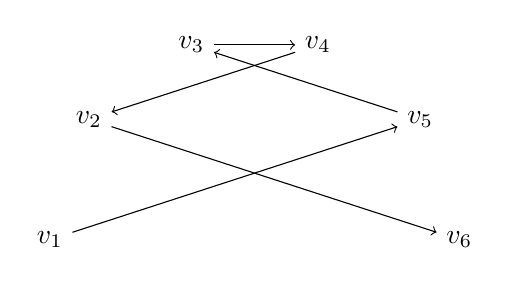
\begin{tikzpicture}[vertex/.style={draw}]
				\foreach \a in {1,...,6}{
						\draw (216-\a*360/10: 2.6cm) node (\a) {$v_\a$};
					}
				\draw[->] (1) -- (5);
				\draw[->] (5) -- (3);
				\draw[->] (3) -- (4);
				\draw[->] (4) -- (2);
				\draw[->] (2) -- (6);
			\end{tikzpicture}
		}
		\caption{Swapping $v_2$ and $v_5$, keeping the order of the nodes in between.}
		\label{fig:03:rialgoreorderkeep}
	\end{subfigure}
	\begin{subfigure}{0.45\textwidth}
		\centering
		\scalebox{0.78}{
			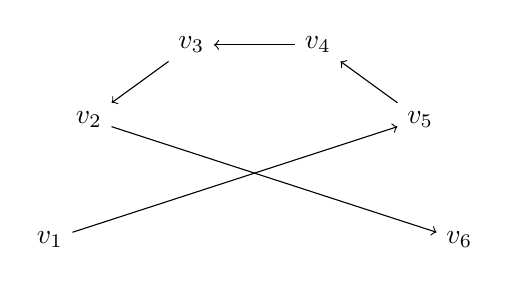
\begin{tikzpicture}[vertex/.style={draw}]
				\foreach \a in {1,...,6}{
						\draw (216-\a*360/10: 2.6cm) node (\a) {$v_\a$};
					}
				\draw[->] (1) -- (5);
				\draw[->] (5) -- (4);
				\draw[->] (4) -- (3);
				\draw[->] (3) -- (2);
				\draw[->] (2) -- (6);
			\end{tikzpicture}
		}
		\caption{Swapping $v_2$ and $v_5$, \emph{reversing} the order of the nodes in between.}
		\label{fig:03:rialgoreorderreverse}
	\end{subfigure}
	\caption{}
	\label{fig:03:rialgoreorder}
\end{wrapfigure}

\subsubsection{Reordering Nodes}
\label{subsubsec:03:reorder}

The first operation is to reorder nodes within a path by swapping two nodes.
While this will not increase a path's score, one hopes that it will reduce the path's total weight.

There are two types of swaps between two nodes $v_i$ and $v_j$.
\begin{enumerate}
	\itemsep0em
	\item Swap $v_i$ and $v_j$ keeping the order of nodes between them.
	\item Swap $v_i$ and $v_j$ and reverse the order of nodes between them.
\end{enumerate}
If any of the two types of swaps decreases the weight, the better swap is applied to the path.

An example path 1-2-3-4-5-6 is depicted in \cref{fig:03:rialgoreorderpath}.
In \cref{fig:03:rialgoreorderkeep}, nodes $v_2$ and $v_5$ are swapped but the order of the nodes in between them is kept as is.
The resulting path is 1-5-3-4-2-6.
In \cref{fig:03:rialgoreorderreverse} the order of the nodes in between is reversed, resulting in the path 1-5-4-3-2-6.

\subsubsection{Introduction of new Nodes}

In contrast to the previous section, this operation does not decrease the weight, but is only interested in increasing score.
Of course, only insertions that do not violate $T_{max}$ are allowed.
If a set of possible insertions is determined, the position that increases the cost the least is chosen.

\subsubsection{Replacing a Node}

This approach inserts an unvisited node into the path while at the same time removing another node from the path.
We choose a node $v_i$ which would be profitable to include in the path.
We then need to find the place in the path in which it would cause the smallest increase in the path's cost.
Then, find a node $v_j$ that if excluded would sufficiently decrease the cost of the path while minimizing the loss in score.
We can now remove $v_j$ from the path and insert $v_i$.
If there is a choice between multiple pairs of nodes, we pick the most profitable pair.

\subsubsection{Generalizing to non-Euclidean inputs}

Since this algorithm does not make any assumptions about its input, except for graph completeness it should work on any graph that is complete.

